\section{Architecture Design}
\label{sec:architecture_design}

The project will consist of a few different subsystems, each serving specialized purposes and communicating in a client-server structure. An overview of the entire structure can be seen in \autoref{fig:arch_design}, and each part will be explained in this section.

\begin{figure}[ht]
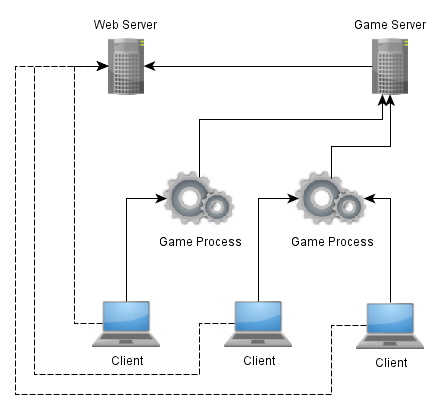
\includegraphics[width=\textwidth]{img/architecture-design.png}
\caption{Architecture Overview}
\label{fig:arch_design}
\end{figure}

\subsection{Distributing Game Data}

All the static data for the game will be distributed by a web server. This includes all of the data needed to execute the game, such as source code and graphics, as well as miscellaneous files, such as game manuals. A database containing user credentials, high scores and other player rankings will also be located on this server.

\subsection{Executing the Game}

The game will be executed on a client. A client is the machine of any user trying to access the game. When started, the client will connect to the web server and request all the static data. When this has been transferred, the client has no more need of the web server. At this point, all of the game logic and graphics will run on the client, making the load on the web server very light, allowing as many players as possible to access the game. Technically, the client could run the game completely autonomously, but since a competitive aspect is desired there is a very serious concern: Cheating.

Any application running locally on a user's machine is prone to manipulation of various kinds. This is especially true for any JavaScript based applications, as most browsers have JavaScript consoles, either built in or using a plugin such as Firebug for Firefox, which allows the user to manipulate the state of the game at any time. This could include changing their score for a better position on a high score table in a single player game, or removing the opponent's cells in a multi player game.

\subsection{Game Validation}

To eliminate the problem of cheating, each game must be validated through a central system, in this case, called the game server. Whenever a client starts a ranked game, either single player or multi player they will have to contact the game server. The game server will then create a process for the player(s) which maintains the state of the game. This requires the game server to have a copy of the implementation of the game logic, to make sure that no data is changed at the wrong time, and every time a client takes an action, it will be validated against the logic in the game server. This includes checking if the users are running valid programs, and that each cell's energy and instruction pointer is set correctly, among other such checks.

At first seems like it could undermine the entire scalability advantage of having all of the game code running on the client. However, there are several things to keep in mind. For example, the game server needs only the game logic, it has no use for any of the graphics, sounds or other static data the client use when running the game. Additionally, only active games are maintained by the game server, players in the game menu and in the program editor (where they are expected spend a considerable amount of the playing time) need not be connected to the game server, as programs will be validated upon game start. Finally, the logic on the game server does not need to run in a browser, so it can be written in a compiled language with higher performance than JavaScript. All in all, a game session on the game server can be a very light process. Should this prove not to be enough, the game server could be replaced with several game servers running the same system, as no data needs to be shared between game sessions in progress, so an almost linear scaling could be achieved.

The last responsibility of the game server is reporting the result of each game to the web server, such that high scores can be updated.

